\documentclass[../../main.tex]{subfiles}

\graphicspath{{../../image/}{../../figure/}}

\begin{document}

\section{梯度计算}\label{section:ch08-梯度计算}

下面让我们为具有任意前馈拓扑结构、任意可微分非线性激活函数和一大类误差函数的通用网络推导出反向传播算法。然后，我们将使用一个简单的分层网络结构（具有单层 S 形隐藏单元以及平方和误差）来说明所得公式。

许多具有实际意义的误差函数（例如由一组独立同分布数据的最大似然定义的误差函数）都包含一些项（其中的每一项对应训练集中的一个数据点）的总和，因此
\begin{align}
E(\mathbf{w})=\sum_{n=1}^{N}E_n(\mathbf{w}).
\label{align:ch08-误差分解}
\end{align}

在此，我们将考虑如何为误差函数中这样一项的 $\nabla E_n(\mathbf{w})$ 求值。这可以直接用于随机梯度下降法，也可以将结果累积到一组训练数据点上，用于批量处理或小批量处理方法。

\subsection{单层网络}\label{subsection:ch08-单层网络}

考虑一个简单的线性模型，其中输出 $y_k$ 是输入变量 $x_i$ 的线性组合，因此
\begin{align}
y_k=\sum_{i}w_{ki}x_i.
\label{align:ch08-单层输出}
\end{align}

对于特定的输入数据点 $n$，平方和误差函数的形式为
\begin{align}
E_n=\frac{1}{2}\sum_{k}\left(y_{nk}-t_{nk}\right)^{2},
\label{align:ch08-单层误差}
\end{align}
其中 $y_{nk}=y_k(\mathbf{x}_n,\mathbf{w})$，$t_{nk}$ 是关联的目标值。该误差函数相对于权重 $w_{ji}$ 的梯度为
\begin{align}
\frac{\partial E_n}{\partial w_{ji}}=\left(y_{nj}-t_{nj}\right)x_{ni}.
\label{align:ch08-单层梯度}
\end{align}

这可以理解为“本地”计算，涉及与链路输出端 $w_{ji}$ 相关的“误差信号” $(y_{nj}-t_{nj})$ 和与链路输入端相关的变量 $x_{ni}$ 的乘积。逻辑斯谛 sigmoid 激活函数与交叉熵误差函数、以及 softmax 激活函数和与之匹配的多元交叉熵误差函数是如何产生类似公式的，参见\cref{subsection:ch05-logistic回归}。接下来，我们将探究这一简单结果如何扩展到更复杂的多层前馈网络情境。

\subsection{一般前馈网络}\label{subsection:ch08-一般前馈网络}

一般来说，前馈网络由一组单元组成，每个单元计算其输入的加权和：
\begin{align}
a_j=\sum_{i}w_{ji}z_i,
\label{align:ch08-预激活}
\end{align}
其中 $z_i$ 是另一个单元的激活值，或是向单元 $j$ 发送连接的输入单元，而 $w_{ji}$ 是与该连接相关的权重。此外，可以通过引入一个额外的单元或输入（激活值固定为 $+1$）来将偏置包含在该总和中，因此我们不需要显式地处理偏置（参见\cref{section:ch06-多层网络}）。在通过非线性激活函数 $h(\cdot)$ 进行转换后，\eqref{align:ch08-预激活}中的和（称为预激活）给出单元 $j$ 的激活值 $z_j$，其形式为
\begin{align}
z_j=h(a_j).
\label{align:ch08-激活}
\end{align}

请注意，\eqref{align:ch08-预激活}中参与求和的一个或多个变量 $z_i$ 可以是一个输入变量。同样，\eqref{align:ch08-激活}中的单元 $j$ 也可以是一个输出变量。

\begin{definition}[计算图]\label{definition:ch08-计算图}
把前馈网络中的每个单元画成一个节点，把每条权重为 $w_{ji}$ 的连接画成从节点 $i$ 指向节点 $j$ 的有向边，所得的有向无环图称为该网络的\textbf{计算图}（computational graph）。在计算图中，节点 $i$ 的激活值 $z_i$ 沿边的方向送入节点 $j$ 并参与\eqref{align:ch08-预激活}的求和，因此\eqref{align:ch08-预激活}与\eqref{align:ch08-激活}就是信息沿边正向流动一次的结果；反过来，若把误差函数对某个节点的预激活的导数看作该节点携带的信号，那么这个信号可以沿边反向送回它的全部前驱节点。
\end{definition}

% SUPPLEMENT: parent=definition:ch08-计算图; kind=motivation; location=紧随其后的 remark（重构新增）
\begin{remark}（重构新增）
计算图之所以值得单独定义，是因为它把“网络里谁影响谁”这件事从公式中剥离出来，只留下节点与有向边。有了它，前向传播与反向传播就不是两套彼此独立的公式，而是同一张图上的两次遍历：一次顺着边的方向求值，一次逆着边的方向累积导数。定义要求图是有向无环图，这保证两次遍历都能按拓扑序进行、不会出现“节点依赖自己”的循环，因而每个节点的量都能由它的前驱（或后继）先算出来；若网络中存在反馈连接，遍历顺序就不再存在，必须改用迭代求解。定义还隐含要求每个节点上的激活函数可微，否则反向遍历时 $\partial z_j/\partial a_j$ 不存在（\eqref{align:ch08-激活}的导数即 $h'(a_j)$）。求值轨迹（参见\cref{section:ch08-自动微分法}）是计算图的一个特例：那里的节点是初等运算而不是网络单元，但“沿边正向求值、反向累积”的结构完全相同，这正是自动微分能够统一处理前向模式与逆模式的原因。
\end{remark}

对于训练集中的每个数据点，我们假设已经向网络提供了相应的输入向量，并通过连续应用\eqref{align:ch08-预激活}和\eqref{align:ch08-激活}计算出了网络中所有隐藏单元和输出单元的激活值。

\begin{definition}[前向传播]\label{definition:ch08-前向传播}
从输入单元出发，沿\cref{definition:ch08-计算图}中边的方向依次对每个单元计算\eqref{align:ch08-预激活}与\eqref{align:ch08-激活}，从而得到网络中所有隐藏单元和输出单元的激活值，这一过程叫作\textbf{前向传播}（forward propagation），因为它可以被视为信息通过网络的前向流动。
\end{definition}

% SUPPLEMENT: parent=definition:ch08-前向传播; kind=motivation; location=紧随其后的 remark（重构新增）
\begin{remark}（重构新增）
前向传播是唯一需要真正“跑一遍网络”的步骤：它把输入 $\mathbf{x}$ 变成输出 $\mathbf{y}$，同时把所有中间激活值 $z_j$ 留在内存中。定义中的“沿边的方向”不是修辞：由于计算图无环，每个单元的预激活只依赖它前驱的激活值，因此可以逐个单元地求值，而不必解联立方程。需要注意，前向传播本身并不涉及误差函数，也不产生任何导数；它只是为反向传播准备好两样东西——各单元的预激活 $a_j$（用于计算 $h'(a_j)$）和各单元的输入 $z_i$（用于计算权重梯度）。这也解释了为什么反向传播的存储开销与前向传播相当：\eqref{align:ch08-权重梯度}需要 $z_i$，\eqref{align:ch08-隐藏误差}需要 $a_j$，二者都必须保留到反向阶段。
\end{remark}

下面让我们来计算 $E_n$ 相对于权重 $w_{ji}$ 的导数。各单元的输出将取决于特定输入数据点 $n$。不过，为了使符号简洁，我们将省略网络变量的下标 $n$。首先要注意的是，$E_n$ 对 $w_{ji}$ 的依赖仅体现在输入 $a_j$ 对单元 $j$ 的求和上。

\begin{proposition}[偏导数的链式法则]\label{proposition:ch08-链式法则}
设误差函数 $E$ 关于所有权重可微，并且 $E$ 对权重的依赖全部通过有限个中间变量 $a_1,\cdots,a_J$（即各单元的预激活）传递。若权重 $w_{ji}$ 只出现在\eqref{align:ch08-预激活}中 $a_j$ 的表达式里，而对其他 $a_l$（$l\neq j$）没有影响，则
\begin{align}
\frac{\partial E}{\partial w_{ji}}=\frac{\partial E}{\partial a_j}\frac{\partial a_j}{\partial w_{ji}}.
\label{align:ch08-链式法则}
\end{align}
若某个权重同时出现在多个预激活的表达式中，则右端应改为对这些预激活求和。
\end{proposition}

\begin{proof}（重构新增）
固定除 $w_{ji}$ 之外的全部权重，把 $E$ 看成 $w_{ji}$ 的一元函数。由\eqref{align:ch08-预激活}，$a_j$ 是 $w_{ji}$ 的可微函数，而其余 $a_l$ 与 $w_{ji}$ 无关，于是复合函数
\begin{align*}
g(t)=E\bigl(a_1,\cdots,a_{j-1},a_j(t),a_{j+1},\cdots,a_J\bigr)
\end{align*}
在 $t=w_{ji}$ 处的导数由一元复合函数求导法则给出：
\begin{align*}
g'(w_{ji})=\frac{\partial E}{\partial a_j}\Big|_{\mathbf{a}}\cdot\frac{\mathrm{d}a_j}{\mathrm{d}w_{ji}}.
\end{align*}
另一方面，$g'(w_{ji})$ 按定义就是 $E$ 沿坐标 $w_{ji}$ 的偏导数 $\partial E/\partial w_{ji}$，而 $\mathrm{d}a_j/\mathrm{d}w_{ji}$ 就是偏导数 $\partial a_j/\partial w_{ji}$，故\eqref{align:ch08-链式法则}成立。若 $w_{ji}$ 同时影响若干个 $a_l$，则 $g$ 是多个一元函数的复合，一元链式法则给出的是各项之和，即右端对全部受影响的 $a_l$ 求和。
\end{proof}

% SUPPLEMENT: parent=proposition:ch08-链式法则; kind=motivation; location=紧随其后的 remark（重构新增）
\begin{remark}（重构新增）
这条法则的内容可以概括为“上游导数乘局部导数”：$\partial E/\partial a_j$ 描述误差函数对单元 $j$ 输出的敏感程度，$\partial a_j/\partial w_{ji}=z_i$ 描述权重对单元 $j$ 预激活的敏感程度，两者相乘即得权重对误差函数的影响。它的条件必须逐条看清。第一，$E$ 与 $a_j$ 都必须可微；对于 ReLU 这类在原点不可微的激活函数，法则在折点处失效，实践中只能取某一侧的导数（次梯度）。第二，命题要求 $w_{ji}$ 只影响一个预激活；深度网络中同一权重通常只属于一条连接，所以这一条自动满足，但若做权重共享（如卷积核在多个位置复用），同一权重就会出现在多个 $a_j$ 中，此时必须求和而不能只取一项，这是实现共享参数网络时最容易出错的地方。第三，法则只用到“局部”信息，不要求知道 $E$ 的全局形式——正是这一点使反向传播可以对任意拓扑的网络逐个单元地递推，而不必展开整个复合函数。
\end{remark}

接下来引入一个有用的符号。

\begin{definition}[误差项]\label{definition:ch08-误差项}
称单元 $j$ 的预激活对误差函数的偏导数为该单元的\textbf{误差}（error），记作
\begin{align}
\delta_j\triangleq\frac{\partial E_n}{\partial a_j},
\label{align:ch08-误差}
\end{align}
其中 $\delta_j$ 通常简称为误差，缘由后续将很快揭晓。
\end{definition}

% SUPPLEMENT: parent=definition:ch08-误差项; kind=motivation; location=紧随其后的 remark（重构新增）
\begin{remark}（重构新增）
把 $\delta_j$ 定义在预激活 $a_j$ 而不是激活值 $z_j$ 上，是一个刻意的选择：$a_j$ 是权重线性进入单元的位置，$\partial a_j/\partial w_{ji}=z_i$ 与单元自身无关，因此所有“与单元有关”的信息都被集中到 $\delta_j$ 里，权重梯度就简化为 $\delta_j z_i$ 这样一个纯粹的乘积。这也解释了“误差”这个名称：对输出单元，$\delta_k=y_k-t_k$ 恰是预测值与目标值之差；对隐藏单元，$\delta_j$ 是把下游各单元的误差按权重 $w_{kj}$ 加权后、再乘上本单元激活函数的斜率 $h'(a_j)$ 得到的量，它不是某个可直接观测的“误差”，而是误差信号反向流经该单元时的强度。注意 $\delta_j$ 与 $\partial E_n/\partial z_j$ 只相差一个因子：$\delta_j=h'(a_j)\,\partial E_n/\partial z_j$，当 $h'(a_j)=0$（例如 tanh 饱和）时该单元对上游完全没有影响，这正是梯度消失现象的来源。
\end{remark}

利用\eqref{align:ch08-预激活}，我们可以写出
\begin{align}
\frac{\partial a_j}{\partial w_{ji}}=z_i.
\label{align:ch08-局部导数}
\end{align}

将\eqref{align:ch08-误差}和\eqref{align:ch08-局部导数}代入\eqref{align:ch08-链式法则}，即得到权重 $w_{ji}$ 的梯度。与它并列，输出单元的误差由误差函数的具体形式直接给出，隐藏单元的误差则可以对\eqref{align:ch08-误差}再用一次链式法则而递归地得到。整理起来，就得到反向传播的四个基本方程。

\begin{theorem}[反向传播的四个基本方程]\label{theorem:ch08-反向传播方程}
在\eqref{align:ch08-预激活}--\eqref{align:ch08-激活}的前馈网络、\eqref{align:ch08-误差}的误差项与\eqref{align:ch08-局部导数}的记号下，给定一个输入数据点，误差函数的全部一阶导数可由下列四个方程求得。
\begin{enumerate}[(i)]
\item\label{item:ch08-输出误差}（输出单元的误差）若输出单元采用与误差函数相匹配的规范连接函数作为激活函数（参见\cref{subsection:ch05-规范连接函数}），则输出单元 $k$ 的误差为
\begin{align}
\delta_k=y_k-t_k,
\label{align:ch08-输出误差}
\end{align}
其中 $y_k$ 是输出单元的激活值，$t_k$ 是相应的目标值；
\item\label{item:ch08-隐藏误差}（隐藏单元的误差）隐藏单元 $j$ 的误差由它向其发送连接的所有单元 $k$ 的误差反向传播得到：
\begin{align}
\delta_j=h'(a_j)\sum_{k}w_{kj}\delta_k,
\label{align:ch08-隐藏误差}
\end{align}
其中求和遍及所有满足“单元 $j$ 向单元 $k$ 发送连接”的单元 $k$，这些单元既可以是其他隐藏单元，也可以是输出单元；
\item\label{item:ch08-权重梯度}（权重的梯度）权重 $w_{ji}$ 的梯度为
\begin{align}
\frac{\partial E_n}{\partial w_{ji}}=\delta_j z_i;
\label{align:ch08-权重梯度}
\end{align}
\item\label{item:ch08-偏置梯度}（偏置的梯度）若把单元 $j$ 的偏置 $b_j$ 显式地写入预激活，即 $a_j=\sum_i w_{ji}z_i+b_j$，则
\begin{align}
\frac{\partial E_n}{\partial b_j}=\delta_j.
\label{align:ch08-偏置梯度}
\end{align}
\end{enumerate}
\end{theorem}

\begin{proof}
下面按推导的先后次序逐条验证这四个方程。

\textbf{权重的梯度\eqref{align:ch08-权重梯度}。}由\cref{proposition:ch08-链式法则}与\eqref{align:ch08-局部导数}，
\begin{align*}
\frac{\partial E_n}{\partial w_{ji}}=\frac{\partial E_n}{\partial a_j}\frac{\partial a_j}{\partial w_{ji}}=\delta_j z_i .
\end{align*}

\textbf{输出单元的误差\eqref{align:ch08-输出误差}。}以平方和误差\eqref{align:ch08-单层误差}与线性输出 $y_k=a_k$ 为例，
\begin{align*}
\delta_k=\frac{\partial E_n}{\partial a_k}=\frac{\partial}{\partial a_k}\left[\frac{1}{2}\sum_{l}\left(y_l-t_l\right)^{2}\right]=\left(y_k-t_k\right)\frac{\partial y_k}{\partial a_k}=y_k-t_k .
\end{align*}
一般地，只要输出单元的激活函数取为与误差函数相匹配的规范连接函数，同样的计算给出同一结果：此时 $\partial E_n/\partial a_k$ 恰好等于“输出值减目标值”。交叉熵与 sigmoid、交叉熵与 softmax 这两种常用组合满足这一条件，具体的验证参见\cref{subsection:ch05-规范连接函数}。

\textbf{隐藏单元的误差\eqref{align:ch08-隐藏误差}。}隐藏单元 $j$ 的预激活 $a_j$ 并不直接出现在误差函数中，它只能通过它所影响的那些预激活 $a_k$（即满足“$j$ 向 $k$ 发送连接”的全部 $k$）去影响 $E_n$。因此对\eqref{align:ch08-误差}再用一次链式法则：
\begin{align*}
\delta_j=\frac{\partial E_n}{\partial a_j}=\sum_{k}\frac{\partial E_n}{\partial a_k}\frac{\partial a_k}{\partial a_j}=\sum_{k}\delta_k\frac{\partial a_k}{\partial a_j},
\end{align*}
这里用到了这样一个事实：只有通过改变变量 $a_k$ 的值，$a_j$ 的变化才会引起误差函数的变化。再由\eqref{align:ch08-预激活}与\eqref{align:ch08-激活}，$a_k=\sum_{l}w_{kl}h(a_l)$，于是
\begin{align*}
\frac{\partial a_k}{\partial a_j}=w_{kj}h'(a_j),
\end{align*}
代回上式即得
\begin{align*}
\delta_j=h'(a_j)\sum_{k}w_{kj}\delta_k .
\end{align*}

\textbf{偏置的梯度\eqref{align:ch08-偏置梯度}（重构新增）。}原书把偏置吸收为激活值恒为 $1$ 的额外输入，没有单列这一方程；若把偏置显式写入预激活，则 $\partial a_j/\partial b_j=1$，于是
\begin{align*}
\frac{\partial E_n}{\partial b_j}=\frac{\partial E_n}{\partial a_j}\frac{\partial a_j}{\partial b_j}=\delta_j .
\end{align*}
若按原书的约定令 $z_0=1$、$b_j=w_{j0}$，则\eqref{align:ch08-权重梯度}在 $z_i=1$ 时也给出\eqref{align:ch08-偏置梯度}，两种写法完全一致。
\end{proof}

% SUPPLEMENT: parent=theorem:ch08-反向传播方程; kind=motivation; location=紧随其后的 remark（重构新增）
\begin{remark}（重构新增）
四个方程可以分成“算误差”与“算梯度”两组：\eqref{align:ch08-输出误差}与\eqref{align:ch08-隐藏误差}负责从输出层出发、逆着计算图逐层求出每个单元的 $\delta$；\eqref{align:ch08-权重梯度}与\eqref{align:ch08-偏置梯度}负责把已经求出的 $\delta$ 就地转换为参数的梯度。这样分组的意义在于复用：同一个 $\delta_j$ 既用于 $j$ 的全部入边权重 $\{w_{ji}\}_i$，也用于偏置 $b_j$，还参与前驱单元的 $\delta$ 的递推，因此不必对每个参数单独做一次前向传播。条件的边界要分清。\eqref{align:ch08-隐藏误差}只要求 $h$ 在 $a_j$ 处可微；若 $h$ 是 ReLU 且在 $a_j=0$ 处不可微，需要约定一个次梯度值，这会使结果依赖于实现约定。\eqref{align:ch08-输出误差}的形式依赖于输出激活函数与误差函数的匹配（规范连接函数）；若换成不匹配的组合，例如 sigmoid 输出配平方和误差，$\delta_k$ 中会多出一个因子 $h'(a_k)$，平方和误差在输出饱和时收敛极慢，这正是分类问题普遍改用交叉熵的原因。\eqref{align:ch08-偏置梯度}只是\eqref{align:ch08-权重梯度}在常数输入下的特例，它说明偏置与权重的梯度在计算上没有本质区别。最后，两个“梯度”方程给出的都是单个数据点的梯度；对整个数据集求和（\eqref{align:ch08-批量梯度}）即得总误差的梯度，但求和必须在 $\delta$ 已经算好之后进行，不能先把各数据点的 $\delta$ 平均掉再反传，否则得到的是平均误差的梯度而不是梯度之和。
\end{remark}

根据\eqref{align:ch08-权重梯度}可知，只需要将权重输出端单元的 $\delta$ 值乘以权重输入端单元的 $z$ 值（其中偏置的 $z=1$），即可得到所需的导数。请注意，这与\eqref{align:ch08-单层梯度}中简单线性模型的形式相同。因此，为了计算导数，我们只需要计算网络中每个隐藏单元和输出单元的 $\delta$ 值，然后应用\eqref{align:ch08-权重梯度}即可。

由此可知，特定隐藏单元的 $\delta$ 值可以通过从网络中较高的单元后向传播误差信息来获得，如\cref{figure:ch08-反向传播示意}所示。

\begin{figure}[htbp]
\centering
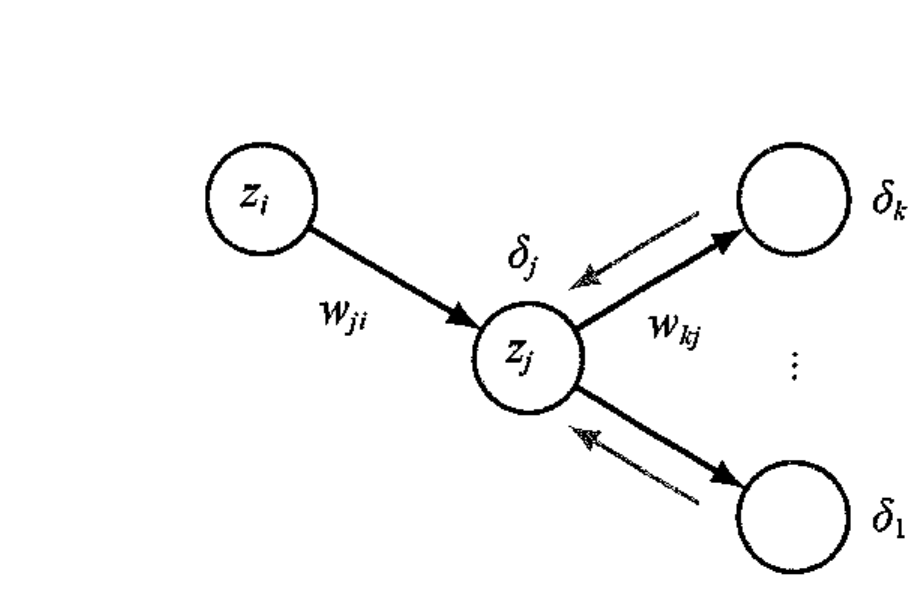
\includegraphics[width=0.40\textwidth]{ch08-fig8-1-backprop.png}
\caption{通过从单元 $k$（单元 $j$ 会向其发送连接）对 $\delta$ 值进行反向传播，计算隐藏单元 $j$ 的 $\delta_j$ 值的示意图。黑色箭头表示前向传播中的信息流方向，红色箭头表示误差信息的反向传播}
\label{figure:ch08-反向传播示意}
\end{figure}

注意，反向传播［\eqref{align:ch08-隐藏误差}］中的求和取自 $w_{kj}$ 上的第一个索引（对应于信息通过网络后向传播），而在前向传播［\eqref{align:ch08-预激活}］中，求和取自第二个索引（见\cref{exercise:ch08-02}）。由于已知输出单元的 $\delta$ 值，因此通过递归应用\eqref{align:ch08-隐藏误差}，我们可以计算前馈网络中所有隐藏单元的 $\delta$ 值，而无须考虑其拓扑结构。算法 8.1 对反向传播做了总结。

\begin{center}
\setlength{\fboxsep}{7pt}%
\fbox{\begin{minipage}{0.78\textwidth}
\centering\textbf{算法 8.1\quad 反向传播}\par
\vspace{5pt}
\begin{flushleft}
\textbf{Input:} 输入向量 $\mathbf{x}_n$\\
\hspace*{1.5em}网络参数 $\mathbf{w}$\\
\hspace*{1.5em}关于输入 $\mathbf{x}_n$ 的误差函数 $E_n(\mathbf{w})$\\
\hspace*{1.5em}激活函数 $h(a)$\\
\textbf{Output:} 误差函数的导数 $\{\partial E_n/\partial w_{ji}\}$\\
// 前向传播\\
\textbf{for} $j\in$ 所有隐藏单元和输出单元 \textbf{do}\\
\hspace*{1.5em}$a_j\leftarrow\sum_i w_{ji}z_i$ \quad // $\{z_i\}$ 包括输入 $\{x_i\}$\\
\hspace*{1.5em}$z_j\leftarrow h(a_j)$ \quad // 激活函数\\
\textbf{end for}\\
// 误差评估\\
\textbf{for} $k\in$ 所有输出单元 \textbf{do}\\
\hspace*{1.5em}$\delta_k\leftarrow\partial E_n/\partial a_k$ \quad // 计算误差\\
\textbf{end for}\\
// 以相反顺序进行反向传播\\
\textbf{for} $j\in$ 所有隐藏单元 \textbf{do}\\
\hspace*{1.5em}$\delta_j\leftarrow h'(a_j)\sum_k w_{kj}\delta_k$ \quad // 递归地进行反向计算\\
\hspace*{1.5em}$\partial E_n/\partial w_{ji}\leftarrow\delta_j z_i$ \quad // 计算导数\\
\textbf{end for}\\
\textbf{return} $\{\partial E_n/\partial w_{ji}\}$
\end{flushleft}
\end{minipage}}
\end{center}

在上述推导中，我们隐式地假设网络中的每个隐藏单元或输出单元都具有相同的激活函数 $h(\cdot)$。不过，只需要跟踪 $h(\cdot)$ 的哪种形式与哪个单元相匹配，就可以轻松地将推导结果拓展到不同的单元，使其拥有单独的激活函数。

对于批量处理方法，对训练集中的每个数据点重复上述步骤，然后对批量处理或小批量处理中的所有数据点求和，即可得到总误差 $E$ 的导数：
\begin{align}
\frac{\partial E}{\partial w_{ji}}=\sum_{n}\frac{\partial E_n}{\partial w_{ji}}.
\label{align:ch08-批量梯度}
\end{align}

\subsection{简单示例}\label{subsection:ch08-简单示例}

上述推导采用了误差函数、激活函数和网络拓扑的一般形式。为了演示反向传播的应用，考虑\cref{figure:ch06-两层网络}所示的两层网络以及平方和误差。

\begin{example}[ 两层网络的误差反向传播]\label{example:ch08-两层网络}
输出单元具有线性激活函数，因此 $y_k=a_k$；而隐藏单元具有 sigmoid 型激活函数，其计算公式为
\begin{align}
h(a)=\tanh(a),
\label{align:ch08-tanh}
\end{align}
其中 $\tanh(a)$ 由\eqref{align:ch06-tanh}定义。该函数的一个有用特征是，它的导数可以用一种特别简单的形式来表示：
\begin{align}
h'(a)=1-h(a)^{2}.
\label{align:ch08-tanh导数}
\end{align}
考虑平方和误差函数，对于数据点 $n$，误差的计算公式为
\begin{align}
E_n=\frac{1}{2}\sum_{k=1}^{K}\left(y_k-t_k\right)^{2},
\label{align:ch08-示例误差}
\end{align}
其中 $y_k$ 是输出单元 $k$ 的激活值，$t_k$ 是特定输入向量 $\mathbf{x}$ 的相应目标值。对于训练集中的每个数据点，首先使用以下方法依次进行前向传播：
\begin{align}
a_j=\sum_{i=0}^{D}w_{ji}^{(1)}x_i,
\label{align:ch08-示例前向1}
\end{align}
\begin{align}
z_j=\tanh(a_j),
\label{align:ch08-示例前向2}
\end{align}
\begin{align}
y_k=\sum_{j=0}^{M}w_{kj}^{(2)}z_j,
\label{align:ch08-示例前向3}
\end{align}
其中 $D$ 是输入向量 $\mathbf{x}$ 的维度，$M$ 是隐藏单元的总数。此外，我们还利用了 $x_0=z_0=1$，以便在权重中包含偏置参数。
\end{example}

\begin{solution}
用以下方法计算每个输出单元的 $\delta$ 值：由\eqref{align:ch08-输出误差}，输出单元为线性激活，故
\begin{align*}
\delta_k=y_k-t_k .
\end{align*}
然后利用如下方法对误差进行反向传播，从而得出隐藏单元的 $\delta$ 值：
\begin{align*}
\delta_j=\left(1-z_j^{2}\right)\sum_{k=1}^{K}w_{kj}^{(2)}\delta_k .
\end{align*}
上式可根据\eqref{align:ch08-隐藏误差}和\eqref{align:ch08-tanh导数}得出：把 $h'(a_j)=1-\tanh^{2}(a_j)=1-z_j^{2}$ 代入\eqref{align:ch08-隐藏误差}，并注意此处单元 $j$ 只向 $K$ 个输出单元发送连接，即得。最后，第一层和第二层权重的导数为
\begin{align*}
\frac{\partial E_n}{\partial w_{ji}^{(1)}}=\delta_j x_i,\qquad
\frac{\partial E_n}{\partial w_{kj}^{(2)}}=\delta_k z_j ,
\end{align*}
它们分别是\eqref{align:ch08-权重梯度}作用于第一层连接（输入端激活值为 $x_i$）与第二层连接（输入端激活值为 $z_j$）的结果。
\end{solution}

\begin{remark}（重构新增）
这个例子之所以选 tanh 与线性输出，是因为这两处导数都能写成闭合而极简的形式：tanh 的导数可以用自身表示（\eqref{align:ch08-tanh导数}），于是反向传播时不必再存储 $a_j$，直接用前向阶段留下的 $z_j$ 即可；线性输出的导数为 $1$，于是输出端不需要额外乘因子，$\delta_k$ 就直接等于残差 $y_k-t_k$。这也说明网络中真正决定反向传播实现细节的只有两件事：每个单元的 $h'(a_j)$ 如何计算，以及输出单元与误差函数是否匹配。条件方面，\eqref{align:ch08-示例前向1}--\eqref{align:ch08-示例前向3}把偏置写成了下标为 $0$ 的权重，因此求和从 $0$ 开始，$w_{j0}^{(1)}$ 与 $w_{k0}^{(2)}$ 就是原来的偏置参数；若按\eqref{align:ch08-偏置梯度}显式处理偏置，则求和应从 $1$ 开始并另外加上 $b_j$，两种写法给出相同的梯度。
\end{remark}

\subsection{数值微分法}\label{subsection:ch08-数值微分}

反向传播最重要的方面之一是计算效率。为此，让我们来看看计算误差函数导数所需的计算操作数是如何随着网络中权重和偏置的总数 $W$ 的变化而变化的。

在 $W$ 足够大的情况下，计算误差函数导数（给定输入数据点）需要 $\mathcal{O}(W)$ 次运算。这是因为除连接非常稀疏的网络外，权重的数量通常远大于单元的数量，因此前向传播的大部分计算量来自\eqref{align:ch08-预激活}中的求和操作，而计算激活函数的工作量却很小。\eqref{align:ch08-预激活}中参与求和的每一项都需要进行一次乘法和一次加法运算，因此总计算成本为 $\mathcal{O}(W)$。

\begin{proposition}[反向传播的计算复杂度]\label{proposition:ch08-反向传播复杂度}
设网络中有 $W$ 个权重与偏置，且有 $U$ 个单元。若 $W$ 足够大（典型情形是 $W$ 远大于 $U$），则给定一个输入数据点，用反向传播计算误差函数关于全部 $W$ 个参数的一阶导数所需的运算次数为 $\mathcal{O}(W)$，即与一次前向传播同一量级。
\end{proposition}

\begin{proof}
一次前向传播的开销由\eqref{align:ch08-预激活}的求和主导：每条连接贡献一次乘法与一次加法，故前向传播需要 $\mathcal{O}(W)$ 次运算；激活函数只对每个单元作用一次，合计 $\mathcal{O}(U)$，在 $W$ 远大于 $U$ 时可并入 $\mathcal{O}(W)$。反向传播分两步。第一步按\eqref{align:ch08-隐藏误差}求各单元的 $\delta$：每个隐单元要对它发出的每条连接做一次乘加，合计仍是每条连接一次，故为 $\mathcal{O}(W)$；第二步按\eqref{align:ch08-权重梯度}与\eqref{align:ch08-偏置梯度}把每个 $\delta$ 乘以对应的 $z_i$，每个参数一次乘法，共 $\mathcal{O}(W)$。三步相加仍为 $\mathcal{O}(W)$，其中常数因子约为前向传播的 $2$ 至 $3$ 倍。
\end{proof}

% SUPPLEMENT: parent=proposition:ch08-反向传播复杂度; kind=motivation; location=紧随其后的 remark（重构新增）
\begin{remark}（重构新增）
\enlargethispage{2\baselineskip}
这条结论是反向传播全部实用价值的来源：它说明“一次前向 + 一次反向”就能拿到全部 $W$ 个偏导数，平均到每个参数只花常数次运算。若改用有限差分法逐个扰动参数，同样的信息需要 $W$ 次前向传播，代价是 $\mathcal{O}(W^{2})$（\cref{proposition:ch08-数值微分复杂度}）。结论中的“$W$ 足够大”不是修辞：当网络极稀疏、$W$ 与 $U$ 同阶甚至更小时，激活函数的 $\mathcal{O}(U)$ 开销不能再被忽略，此时 $\mathcal{O}(W)$ 的写法应理解为 $\mathcal{O}(W+U)$。另外，这里的计数只统计算术运算，不统计访存：实际实现中反向传播常常受内存带宽限制，实测加速比往往低于运算次数的比值，这也是工程上要尽量让中间结果留在高速缓存中的原因。
\end{remark}

计算误差函数导数的另一种反向传播方法是使用有限差分法。具体做法是依次扰动每个权重，并利用该表达式近似求导来实现：
\begin{align}
\frac{\partial E_n}{\partial w_{ji}}=\frac{E_n\left(w_{ji}+\varepsilon\right)-E_n\left(w_{ji}\right)}{\varepsilon}+\mathcal{O}(\varepsilon),
\label{align:ch08-有限差分}
\end{align}
其中 $\varepsilon\ll1$。在软件模拟中，可以通过将 $\varepsilon$ 最小化来提高导数近似值的精度，直到出现数值舍入问题为止。使用对称中心差分法可以显著提高有限差分法的精度，形式如下：
\begin{align}
\frac{\partial E_n}{\partial w_{ji}}=\frac{E_n\left(w_{ji}+\varepsilon\right)-E_n\left(w_{ji}-\varepsilon\right)}{2\varepsilon}+\mathcal{O}\left(\varepsilon^{2}\right).
\label{align:ch08-中心差分}
\end{align}

在这种情况下，正如\eqref{align:ch08-中心差分}右侧的Taylor展开所验证的，$\mathcal{O}(\varepsilon)$ 修正被抵消了，因此残差修正为 $\mathcal{O}(\varepsilon^{2})$（见\cref{exercise:ch08-03}）。但请注意，计算步骤的数量相比\eqref{align:ch08-有限差分}增加了大约一倍。\cref{figure:ch08-数值微分误差}显示了利用有限差分法［\eqref{align:ch08-有限差分}］和对称中心差分法［\eqref{align:ch08-中心差分}］对梯度进行数值计算的结果与分析结果之间的误差。

\begin{figure}[htbp]
\centering
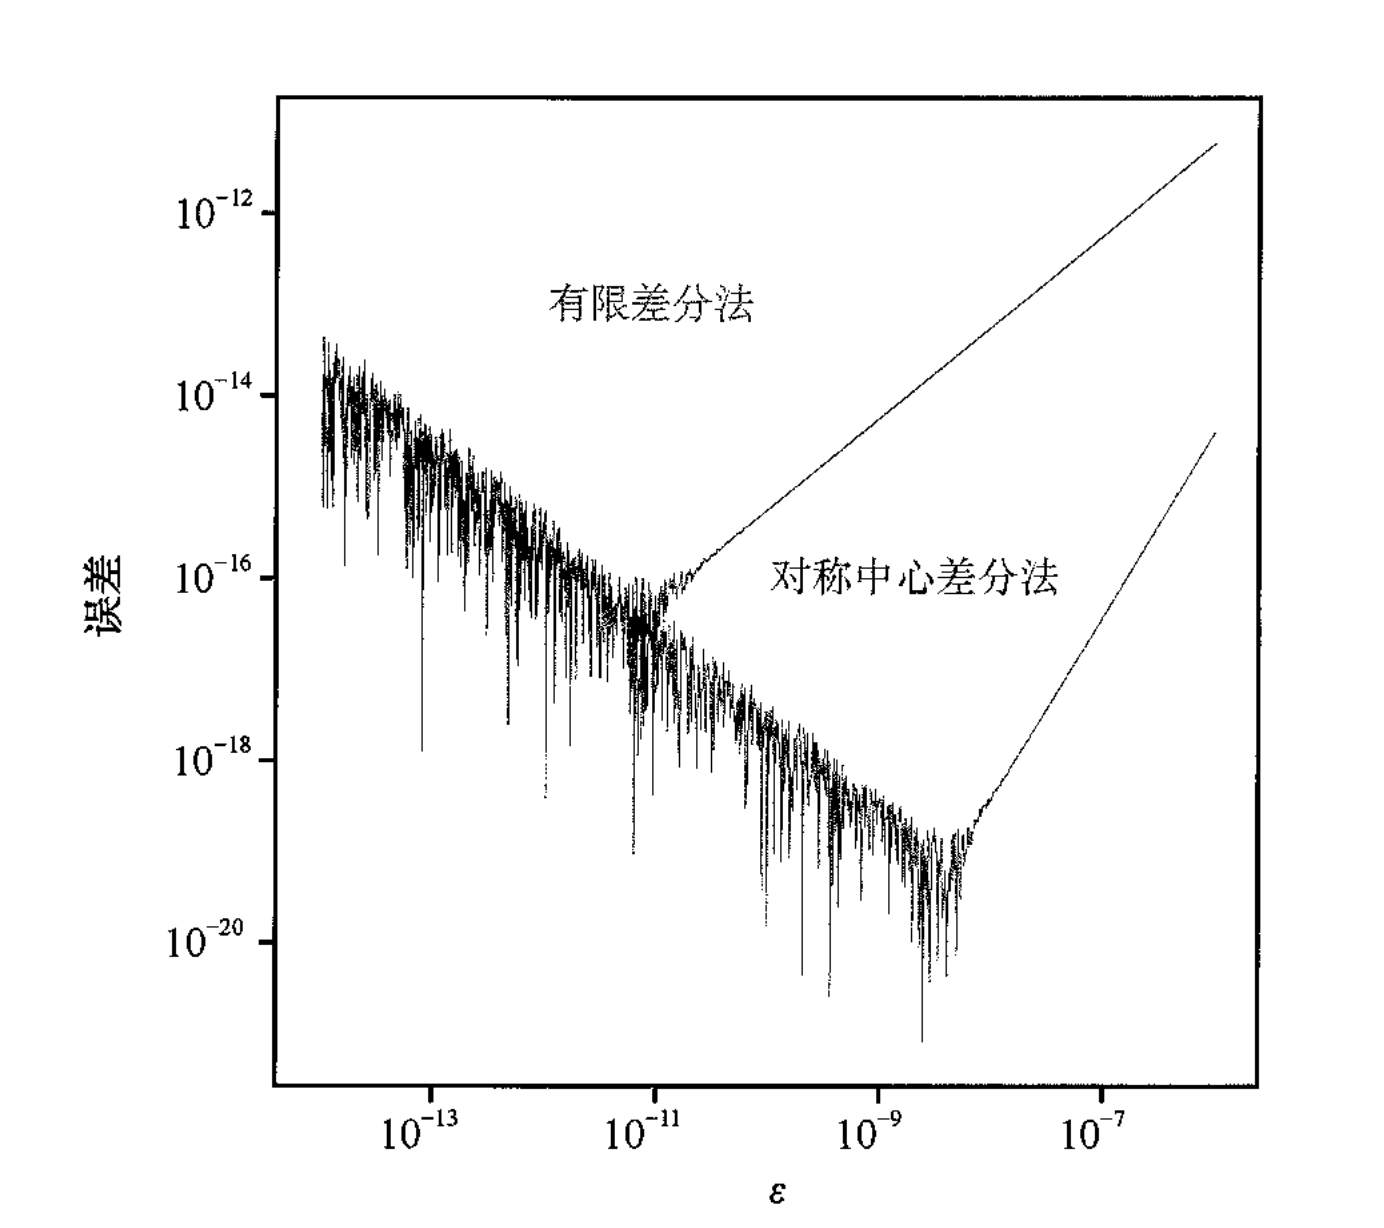
\includegraphics[width=0.62\textwidth]{ch08-fig8-2-numeric-diff.png}
\caption{红色曲线显示了使用有限差分法对梯度进行数值计算的结果与分析结果之间的误差。随着 $\varepsilon$ 不断减小，误差呈线性减小，且由于坐标轴是对数，因此这代表了一种幂律行为。红色曲线的斜率为 $1$，这表明误差为 $\mathcal{O}(\varepsilon)$。在某一点上，所计算的梯度达到数值四舍五入的极限，且 $\varepsilon$ 的进一步减小会导致出现一条噪声线，该噪声线同样遵循幂律，但误差会随着 $\varepsilon$ 的减小而增大。蓝色曲线显示了使用对称中心差分法对梯度进行数值计算的结果与分析结果之间的误差。与有限差分法相比，对称中心差分法的误差要小得多，而且蓝色曲线的斜率为 $2$，这表明误差为 $\mathcal{O}(\varepsilon^{2})$}
\label{figure:ch08-数值微分误差}
\end{figure}

数值微分法的主要问题是失去了非常理想的 $\mathcal{O}(W)$ 缩放。每次前向传播需要执行 $\mathcal{O}(W)$ 个步骤，而网络中有 $W$ 个权重，每个权重都必须单独扰动，因此总计算成本为 $\mathcal{O}(W^{2})$。

\begin{proposition}[数值微分的计算复杂度]\label{proposition:ch08-数值微分复杂度}
用有限差分法\eqref{align:ch08-有限差分}或中心差分法\eqref{align:ch08-中心差分}计算误差函数关于全部 $W$ 个参数的梯度，需要 $\mathcal{O}(W^{2})$ 次运算，即比反向传播贵一个因子 $W$。
\end{proposition}

\begin{proof}
有限差分\eqref{align:ch08-有限差分}每估计一个参数的偏导数需要两次误差函数求值（一次在原参数处、一次在扰动后的参数处），中心差分\eqref{align:ch08-中心差分}需要两次扰动求值；无论哪一种，对全部 $W$ 个参数逐一处理都要进行 $\Theta(W)$ 次误差函数求值。每次求值都是一次前向传播，代价为 $\mathcal{O}(W)$，故总代价为 $\mathcal{O}(W)\times\mathcal{O}(W)=\mathcal{O}(W^{2})$。中心差分只把常数因子提高约一倍，不改变量级。
\end{proof}

% SUPPLEMENT: parent=proposition:ch08-数值微分复杂度; kind=motivation; location=紧随其后的 remark（重构新增）
\begin{remark}（重构新增）
$\mathcal{O}(W^{2})$ 与 $\mathcal{O}(W)$ 的差别不是常数因子，而是量级：当 $W$ 达到 $10^{6}$ 时，两者相差一百万倍，因此把数值微分当作训练算法在实际中不可行。还要注意近似精度与舍入误差的权衡：\eqref{align:ch08-有限差分}的截断误差为 $\mathcal{O}(\varepsilon)$，\eqref{align:ch08-中心差分}为 $\mathcal{O}(\varepsilon^{2})$，减小 $\varepsilon$ 似乎总能提高精度；但 $\varepsilon$ 小到一定程度后，$E_n(w_{ji}+\varepsilon)-E_n(w_{ji})$ 是两个相近数之差，舍入误差被 $\varepsilon$ 放大，总误差随 $\varepsilon$ 减小反而上升——\cref{figure:ch08-数值微分误差}中红色曲线与蓝色曲线在极小 $\varepsilon$ 处的噪声线正是这一现象。因此中心差分除了公式本身的二阶精度，还能把“精度开始劣化”的 $\varepsilon$ 推得更小。它真正的用途不是训练，而是检验：把反向传播或自动微分得到的导数与中心差分的结果比较，可以在不重写反向代码的前提下发现实现错误，这也是本书建议的调试手段。
\end{remark}

不过，数值微分法在实践中也能发挥重要作用，因为将直接实现反向传播或自动微分法计算出的导数与使用中心差分法计算出的导数进行比较，可以有力地检验软件的正确性。

\subsection{Jacobi矩阵}\label{subsection:ch08-Jacobi矩阵}

我们已经了解了如何通过网络反向传播误差来获得误差函数相对于权重的导数。反向传播也可用于计算其他导数。在此，我们对Jacobi矩阵进行求值，其元素由网络输出相对于输入的导数给出。

\begin{definition}[Jacobi矩阵]\label{definition:ch08-Jacobi矩阵}
设网络输出 $y_k$ 与输入 $x_i$ 均可微，则称由网络输出相对于输入的导数构成的矩阵
\begin{align}
J_{ki}=\frac{\partial y_k}{\partial x_i}
\label{align:ch08-Jacobi}
\end{align}
为网络所表示函数的\textbf{Jacobi矩阵}（Jacobian matrix），其中每个导数都是在所有其他输入值保持不变的情况下求得的。
\end{definition}

% SUPPLEMENT: parent=definition:ch08-Jacobi矩阵; kind=motivation; location=紧随其后的 remark（重构新增）
\begin{remark}（重构新增）
Jacobi矩阵回答的是与梯度不同的问题：梯度问“参数怎样变能使误差下降”，Jacobi矩阵问“输入怎样变会使输出怎样变”。它是一个 $K\times D$ 的矩阵（$K$ 为输出维数、$D$ 为输入维数），而不是一个与参数同维的向量，因此“反向传播能算Jacobi矩阵”并不是同义反复——它需要把误差反向传播的程序改造成对每个输出单元分别反向一次的循环。定义要求 $y_k$ 对 $x_i$ 可微，这排除了含硬阈值或取整操作的网络；定义还强调“其他输入保持不变”，即 $J_{ki}$ 是偏导数而不是全导数，若输入之间存在相关性（例如做了归一化），改变 $x_i$ 时其他输入并不会真的保持不变，此时用\eqref{align:ch08-Jacobi扰动}解释灵敏度必须谨慎。由于网络映射是非线性的，$J$ 依赖于具体的输入点，必须在每个新输入处重新计算。
\end{remark}

如\cref{figure:ch08-模块化}所示，Jacobi矩阵在由多个不同模块构建的系统中发挥着重要作用。每个模块都可以包含一个固定的或可学习的函数，该函数可以是线性的或非线性的，但必须是可微分的。假设我们希望最小化\cref{figure:ch08-模块化}中与参数 $\mathbf{w}$ 有关的误差函数 $E$，该误差函数的导数为
\begin{align}
\frac{\partial E}{\partial\mathbf{w}}=\sum_{k,j}\frac{\partial E}{\partial y_k}\frac{\partial y_k}{\partial z_j}\frac{\partial z_j}{\partial\mathbf{w}}.
\label{align:ch08-模块链式}
\end{align}

\begin{figure}[htbp]
\centering
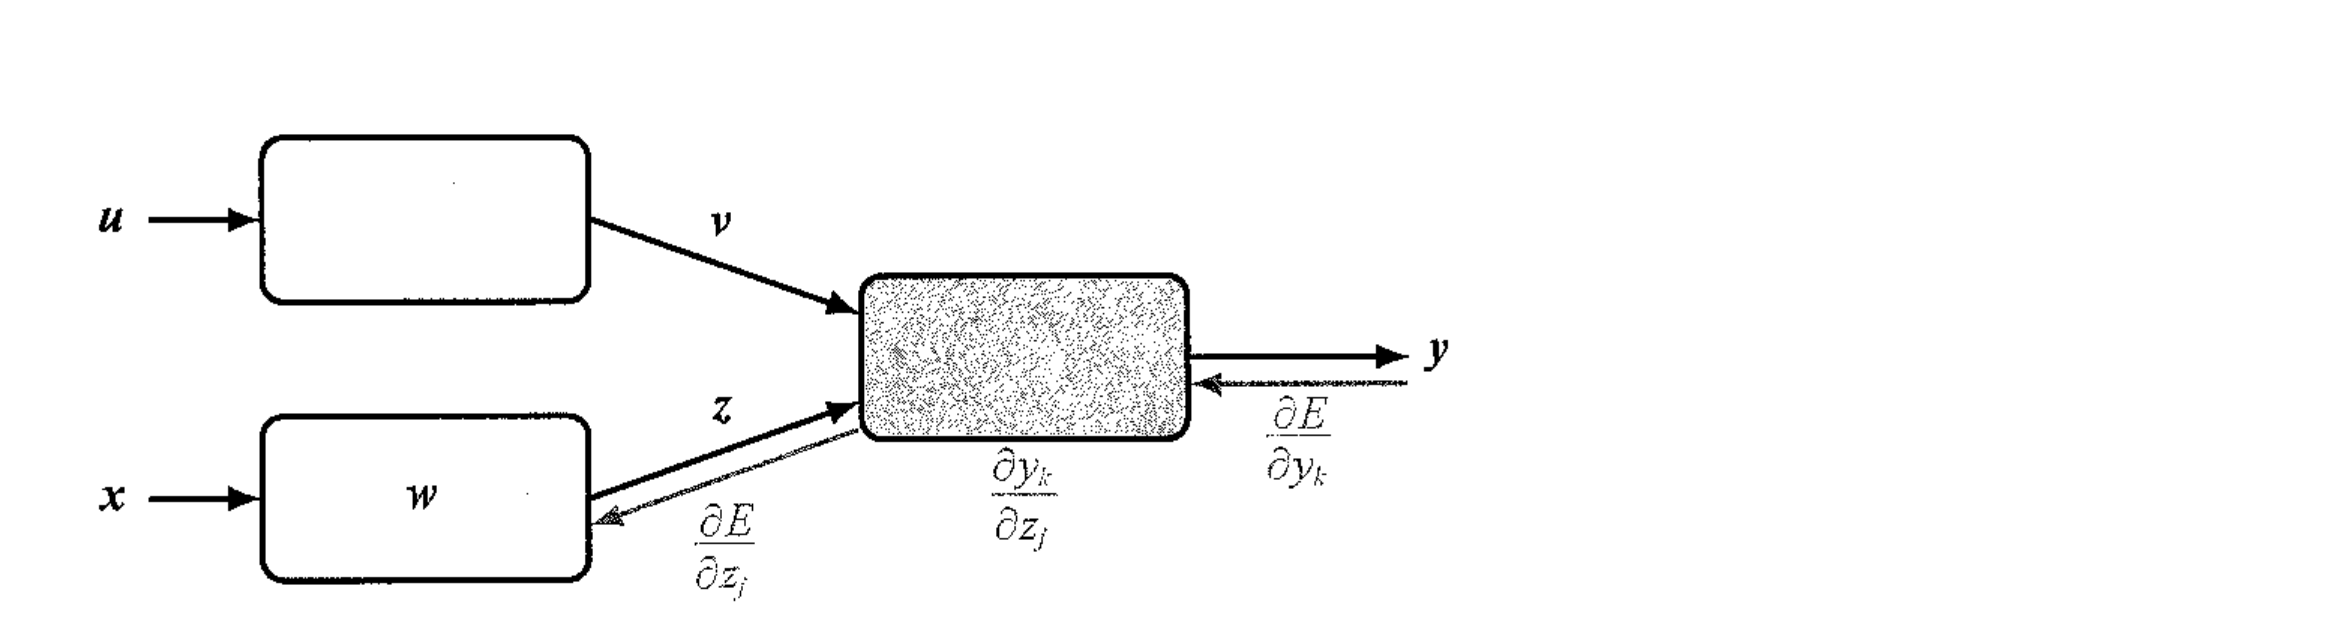
\includegraphics[width=0.72\textwidth]{ch08-fig8-3-modular.png}
\caption{模块化深度学习架构示意图，其中Jacobi矩阵可用于将误差信号从输出反向传播至系统的早期模块}
\label{figure:ch08-模块化}
\end{figure}

\cref{figure:ch08-模块化}中红色模块所代表的Jacobi矩阵出现在\eqref{align:ch08-模块链式}右侧的中间项。

由于Jacobi矩阵度量了输出变量对每个输入变量变化的局部灵敏度，因此它还允许与输入相关的任何已知误差 $\Delta x_i$ 通过经训练的网络进行传播，从而预估它们对输出误差的贡献 $\Delta y_k$：
\begin{align}
\Delta y_k\approx\sum_{i}\frac{\partial y_k}{\partial x_i}\Delta x_i.
\label{align:ch08-Jacobi扰动}
\end{align}

这里假设 $|\Delta x_i|$ 很小。一般来说，训练后的神经网络所代表的网络映射是非线性的，因此Jacobi矩阵的元素不是常数，而取决于所使用的特定输入向量。因此，\eqref{align:ch08-Jacobi扰动}只对输入的微小扰动有效，而且必须为每个新输入向量重新计算Jacobi矩阵。

我们可以使用反向传播程序来计算Jacobi矩阵，该程序与前面计算误差函数相对于权重的导数的程序类似。首先写下元素 $J_{ki}$，形式如下：
\begin{align}
J_{ki}=\frac{\partial y_k}{\partial x_i}=\sum_{j}\frac{\partial y_k}{\partial a_j}\frac{\partial a_j}{\partial x_i}
=\sum_{j}w_{ji}\frac{\partial y_k}{\partial a_j},
\label{align:ch08-Jacobi链式}
\end{align}
其中使用了\eqref{align:ch08-预激活}。\eqref{align:ch08-Jacobi链式}中的求和操作涉及所有单元 $j$（例如前面提到的分层拓扑结构中第一隐藏层的所有单元），且输入单元 $i$ 向单元 $j$ 发送连接。导数 $\partial y_k/\partial a_j$ 的递归反向传播公式如下：
\begin{align}
\frac{\partial y_k}{\partial a_j}=\sum_{l}\frac{\partial y_k}{\partial a_l}\frac{\partial a_l}{\partial a_j}
=h'(a_j)\sum_{l}w_{lj}\frac{\partial y_k}{\partial a_l},
\label{align:ch08-Jacobi递归}
\end{align}
其中的求和操作涉及所有单元 $l$，且单元 $j$ 向单元 $l$ 发送连接（对应于 $w_{lj}$ 的第一个索引）。我们再次使用了\eqref{align:ch08-预激活}和\eqref{align:ch08-激活}。这种反向传播从输出单元开始，所需导数可直接从输出单元激活函数的函数形式中得到。对于线性输出单元，我们可以得出
\begin{align}
\frac{\partial y_k}{\partial a_l}=\delta_{kl},
\label{align:ch08-线性输出Jacobi}
\end{align}
其中 $\delta_{kl}$ 是单位矩阵的元素，定义如下：
\begin{align}
\delta_{kl}=\begin{cases}
1, & k=l,\\
0, & \text{其他}.
\end{cases}
\label{align:ch08-克罗内克}
\end{align}

如果我们在每个输出单元上都有独立的逻辑斯谛 sigmoid 激活函数（参见\cref{section:ch03-指数族分布}），则有
\begin{align}
\frac{\partial y_k}{\partial a_l}=\delta_{kl}\,\sigma'(a_l).
\label{align:ch08-sigmoidJacobi}
\end{align}
而对于 softmax 输出（参见\cref{section:ch03-指数族分布}），可以得出
\begin{align}
\frac{\partial y_k}{\partial a_l}=\delta_{kl}\,y_k-y_k y_l.
\label{align:ch08-softmaxJacobi}
\end{align}

我们可以将Jacobi矩阵的计算程序总结如下。首先，应用与输入空间（在该空间中需要计算Jacobi矩阵）中的点相对应的输入向量，并按照常规方法进行前向传播，以得到网络中所有隐藏单元和输出单元的状态。接下来，对于Jacobi矩阵中与输出单元 $k$ 相对应的每一行 $k$，使用递归关系式\eqref{align:ch08-Jacobi递归}，从\eqref{align:ch08-线性输出Jacobi}、\eqref{align:ch08-sigmoidJacobi}或\eqref{align:ch08-softmaxJacobi}开始，对网络中的所有隐藏单元进行反向传播。最后，使用\eqref{align:ch08-Jacobi链式}对输入进行反向传播。Jacobi矩阵也可以用另一种前向传播形式来计算，其推导方法与此处的反向传播方法类似（见\cref{exercise:ch08-05}）。

同样，此类算法的实现可以用形式如下的数值微分来检验：
\begin{align}
\frac{\partial y_k}{\partial x_i}=\frac{y_k\left(x_i+\varepsilon\right)-y_k\left(x_i-\varepsilon\right)}{2\varepsilon}+\mathcal{O}\left(\varepsilon^{2}\right).
\label{align:ch08-Jacobi数值}
\end{align}
对于有 $D$ 个输入的网络来说，这涉及 $2D$ 次前向传播，因此总共需要 $\mathcal{O}(DW)$ 个步骤。

\subsection{黑塞矩阵}\label{subsection:ch08-黑塞矩阵}

我们已经展示了如何利用反向传播来获得误差函数相对于网络权重的一阶导数。反向传播也可用于计算误差的二阶导数，表达式如下
\begin{align}
\frac{\partial^{2}E}{\partial w_{ji}\partial w_{lk}}
\label{align:ch08-二阶导数}
\end{align}

方便起见，我们通常将所有权重和偏置参数视为单个向量（用 $\mathbf{w}$ 表示）的元素 $w_i$。

\begin{definition}[黑塞矩阵]\label{definition:ch08-黑塞矩阵}
设误差函数 $E(\mathbf{w})$ 关于参数向量 $\mathbf{w}=(w_1,\cdots,w_W)^{\mathsf T}$ 二阶可微。此时二阶导数构成\textbf{黑塞矩阵}（Hessian matrix）$\mathbf{H}$ 的元素
\begin{align}
H_{ij}=\frac{\partial^{2}E}{\partial w_i\partial w_j},
\label{align:ch08-黑塞}
\end{align}
其中 $i,j\in\{1,\cdots,W\}$，$W$ 是权重和偏置的总数。
\end{definition}

% SUPPLEMENT: parent=definition:ch08-黑塞矩阵; kind=motivation; location=紧随其后的 remark（重构新增）
\begin{remark}（重构新增）
黑塞矩阵把误差曲面在一点处的全部二阶信息打包成一个 $W\times W$ 的对称矩阵：对角元 $H_{ii}$ 是沿坐标方向的曲率，非对角元 $H_{ij}$ 刻画两个方向之间的耦合。它与\cref{definition:ch08-Jacobi矩阵}的区别在于对谁求导：Jacobi矩阵对输入求导，黑塞矩阵对参数求二阶导，因此后者的规模由参数个数决定，在深度网络中可达 $10^{6}\times10^{6}$，显式存储都不可能，更不用说求逆。定义要求 $E$ 二阶可微，这保证 $H_{ij}=H_{ji}$；若只二阶可微而不连续，混合偏导数可能不相等，$\mathbf{H}$ 就不对称，基于 $\mathbf{H}$ 的优化算法（Newton 法、共轭梯度）所依赖的性质也随之失效。$\mathbf{H}$ 的用途有三类：判断驻点的类型（正定、负定、不定分别对应极小、极大、鞍点）、构造二次近似以加速优化、以及在Bayes近似中充当后验精度的度量。
\end{remark}

基于误差表面二阶特性的考虑，黑塞矩阵出现在了用于训练神经网络的几种非线性优化算法中（Bishop, 2006）。此外，它还在神经网络的某些Bayes处理中发挥作用（MacKay, 1992; Bishop, 2006），并用于降低大语言模型中权重的精度，从而减少内存占用（Shen et al., 2019）。

在黑塞矩阵的众多应用中，评估黑塞矩阵的效率是十分重要的。如果网络中有 $W$ 个参数（权重和偏置），那么黑塞矩阵的维度为 $W\times W$，因此对于数据集中的每个数据点，计算黑塞矩阵所需的计算量将缩放为 $\mathcal{O}(W^{2})$（见\cref{exercise:ch08-06}）。通过扩展反向传播程序（Bishop, 1992），可以有效地计算黑塞矩阵，缩放比例实际为 $\mathcal{O}(W^{2})$。有时，我们并非直接需要黑塞矩阵，而只需要黑塞矩阵与某个向量 $\mathbf{v}$ 的乘积 $\mathbf{v}^{\mathsf T}\mathbf{H}$；通过扩展反向传播程序，我们可以在 $\mathcal{O}(W)$ 个步骤内高效地计算出该乘积（Møller, 1993; Pearlmutter, 1994）。

由于神经网络可能包含数百万个甚至数十亿个参数，因此对许多模型的全黑塞矩阵进行计算，甚至只进行存储，都是不可行的。由于计算量被缩放为 $\mathcal{O}(W^{3})$，求黑塞矩阵的逆将变得更加困难。业内人士对寻找有效的全黑塞矩阵近似值很感兴趣。

一种近似法是只对黑塞矩阵的对角元素进行计算，并隐式地将非对角元素设为零。这需要 $\mathcal{O}(W)$ 的存储空间，并允许在 $\mathcal{O}(W)$ 个步骤内进行求逆，但仍需要 $\mathcal{O}(W^{2})$ 个计算步骤（Ricotti, Ragazzini, and Martinelli, 1988），不过通过进一步近似，计算步骤可以减少到 $\mathcal{O}(W)$ 个（Becker and LeCun, 1989; LeCun, Denker, and Solla, 1990）。但实际上，黑塞矩阵通常具有重要的非对角项，因此必须谨慎对待这一近似值。

另一种更有说服力的方法是外积近似法，原理如下。考虑使用平方和误差函数的回归应用，平方和误差函数如下：
\begin{align}
E=\frac{1}{2}\sum_{n=1}^{N}\left(y_n-t_n\right)^{2},
\label{align:ch08-平方和误差}
\end{align}
其中只使用了一个单一输出，以保持符号简洁（扩展到多个输出也很简单）。然后写下黑塞矩阵（见\cref{exercise:ch08-08}），形式如下：
\begin{align}
\mathbf{H}=\nabla\nabla E=\sum_{n=1}^{N}\nabla y_n\left(\nabla y_n\right)^{\mathsf T}+\sum_{n=1}^{N}\left(y_n-t_n\right)\nabla\nabla y_n,
\label{align:ch08-黑塞展开}
\end{align}
其中 $\nabla$ 表示相对于 $\mathbf{w}$ 的梯度。如果网络已在数据集上经过训练，则输出 $y_n$ 将非常接近目标值 $t_n$，\eqref{align:ch08-黑塞展开}中末尾的项很小，可以忽略不计。不过，从更广泛的意义上讲，根据以下推论，忽略这一项可能是合适的。回顾\cref{section:ch04-决策理论}，最优函数是使平方和损失最小化的目标数据的条件平均值。量 $(y_n-t_n)$ 是一个均值为零的随机变量。如果假设它的值与\eqref{align:ch08-黑塞展开}右侧二阶导数项的值无关，那么在对 $n$ 求和时，整个导数项的平均值将为零（见\cref{exercise:ch08-09}）。

忽略\eqref{align:ch08-黑塞展开}右侧的二阶导数项，即可得到 Levenberg--Marquardt 近似法，也叫作外积近似法，因为黑塞矩阵是由向量的外积之和构成的。

\begin{definition}[外积近似（Levenberg--Marquardt 近似）]\label{definition:ch08-外积近似}
对形如\eqref{align:ch08-平方和误差}的平方和误差函数，略去\eqref{align:ch08-黑塞展开}中的二阶导数项，用一阶导数（梯度）的外积之和作为黑塞矩阵的近似：
\begin{align}
\mathbf{H}\approx\sum_{n=1}^{N}\nabla a_n\nabla a_n^{\mathsf T}.
\label{align:ch08-外积近似}
\end{align}
这一近似称为\textbf{外积近似}（outer product approximation），也称 Levenberg--Marquardt 近似。
\end{definition}

% SUPPLEMENT: parent=definition:ch08-外积近似; kind=motivation; location=紧随其后的 remark（重构新增）
\begin{remark}（重构新增）
外积近似用“梯度的外积”代替“二阶导数”，好处是只依赖一阶信息：一阶导数已由反向传播在 $\mathcal{O}(W)$ 内算出，再对每个数据点做一次外积，就得到 $\mathbf{H}$ 的全部元素，总代价 $\mathcal{O}(W^{2})$，与显式求二阶导的代价同阶但常数小得多；而且每个外积 $\nabla a_n\nabla a_n^{\mathsf T}$ 都是半正定的秩一矩阵，故近似后的 $\mathbf{H}$ 自动半正定，这使基于它的迭代（如 Levenberg--Marquardt 的阻尼步）不会因负曲率而失稳。代价是它丢掉了二阶项，因此近似的好坏取决于 $|y_n-t_n|$ 是否足够小：网络训练充分时残差接近零，近似成立；网络远未训练好时残差很大，二阶项不可忽略，此时用外积近似可能严重低估曲率（见\cref{exercise:ch08-09}的讨论）。还要注意，\eqref{align:ch08-外积近似}写的是 $\nabla a_n$ 而不是 $\nabla y_n$，这是因为在平方和误差的标准配置中输出单元是线性的，$y_n=a_n$，两者相同；若输出单元带非线性激活，则必须换回 $\nabla y_n$。
\end{remark}

求黑塞矩阵的外积近似值非常简单，因为仅涉及误差函数的一阶导数，使用标准反向传播法即可在 $\mathcal{O}(W)$ 个步骤内高效地计算出误差函数的一阶导数。而通过进行简单的乘法运算，只需要 $\mathcal{O}(W^{2})$ 个步骤即可求出矩阵的元素。需要强调的是，这种近似法可能只适用于经过适当训练的网络，且对于一般的网络映射，\eqref{align:ch08-黑塞展开}右侧的二阶导数项通常是不可忽略的。

对于具有逻辑斯谛 sigmoid 输出单元激活函数的网络，其交叉熵误差函数的相应近似值为
\begin{align}
\mathbf{H}\approx\sum_{n=1}^{N}y_n\left(1-y_n\right)\nabla a_n\nabla a_n^{\mathsf T}.
\label{align:ch08-外积交叉熵}
\end{align}

对于具有 softmax 输出单元激活函数的多类网络，均可以得到类似的结果（见\cref{exercise:ch08-11}）。外积近似法还可用于开发一种高效的序列程序，用于近似黑塞矩阵的逆（Hassibi and Stork, 1993）（见\cref{exercise:ch08-12}）。

\end{document}
